\documentclass[12pt]{article}

\usepackage[utf8]{inputenc}
\usepackage[T1]{fontenc}
\usepackage[french]{babel}
\usepackage{hyperref}
\usepackage{graphicx}
\usepackage{listings}
\usepackage[linesnumbered,ruled,french,onelanguage]{algorithm2e}
\lstset{numbers=left, numberstyle=\tiny, stepnumber=1, numbersep=6pt}
\makeatletter 
\g@addto@macro{\@algocf@init}{\SetKwInput{KwOut}{Sortie}}
\makeatother
\title{Aide à la Décision - Othello}
\author{Antonin Boyon \and Quentin Legot \and Arthur Page}
\date{\today}

\begin{document}

\maketitle
\thispagestyle{empty}
\setcounter{page}{0}
\newpage

\tableofcontents
\newpage

\section{Introduction}

Le but de notre projet était de concevoir un algorithme de recherche performant sur un jeu d' \textit{Othello}. Le jeu est le plus abstrait possible, la partie nous intéressant étant la réalisation d'un algorithme de recherche efficace. Il est ainsi impossible de jouer au jeu, on ne peut que regarder le résultat d'une partie entre deux joueurs artificiels.\\
Une fois le jeu et l'algorithme de recherche implémentés, nous serons en mesure d'analyser ce dernier pour définir ses paramètres de fonctionnement optimaux. Nous aborderons dans un premier temps l'implémentation du jeu, puis celle de l'algorithme et enfin la présentation et l'analyse des mesures observées.

\section{L'algorithme de recherche}
\subsection{Algorithme de base}

Nous avons utilisé un algorithme Negamax pour résoudre le problème.

\lstinputlisting[language=Java]{NegamaxPlayer.txt}

\subsection{Algorithme d'élagage}

\lstinputlisting[language=Java]{AlphaBetaPlayer.txt}

\section{Mesures}

\subsection{Présentation}

Les graphiques qui vont suivre ont été conçus à l’aide des algorithmes AlphaBeta et Negamax.\\
Ils sont l’objet de comparaisons entre les algorithmes, en fonction de leur type ou du joueur concerné (premier ou second joueur).\\
Ils traduisent la complexité de l’algorithmes (le nombre de nœuds traversés) au fur et à mesure des tours de la partie.\\
Le premier joueur est associé à la courbe rouge et le deuxième à la bleue.\\
La profondeur de recherche des deux joueurs sera toujours la même.\\

Tout les tests incluant un temps ont été fait sur la même machine et en même temps: Raspberry pi 3 avec un processeur Quad Core 1.2GHz 64bit sous Raspbian OS 32 bits sans Bureau.
\newpage

\begin{figure}[!h]
   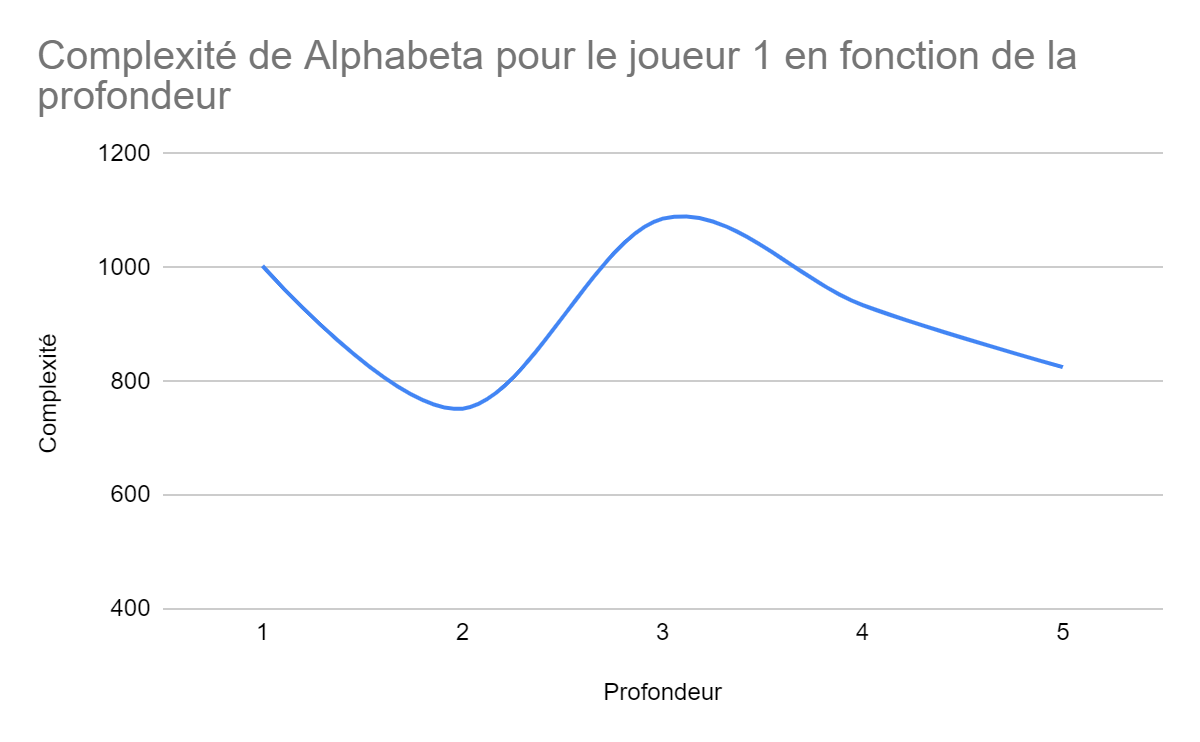
\includegraphics[width=\textwidth]{alphabeta.png}
\end{figure}

\begin{figure}[!h]
   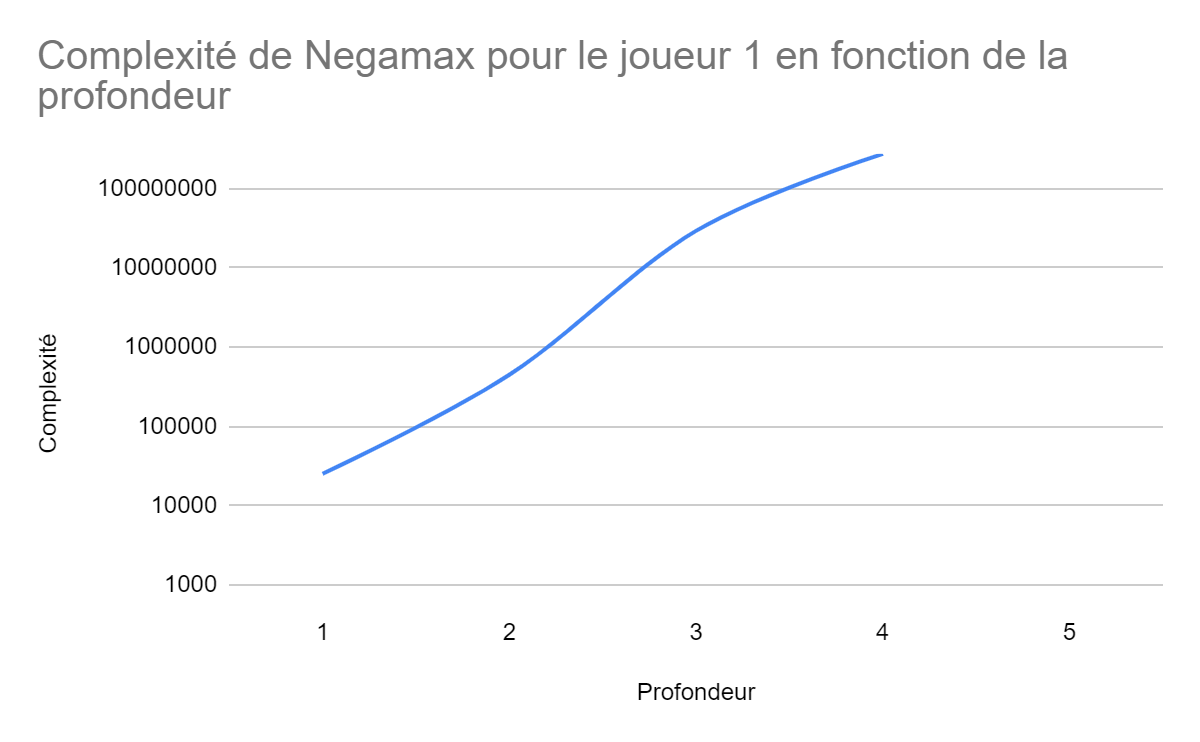
\includegraphics[width=\textwidth]{negamax.png}
\end{figure}

\subsection{AlphaBeta}

\subsubsection{Profondeur 1}

\begin{figure}[!h]
   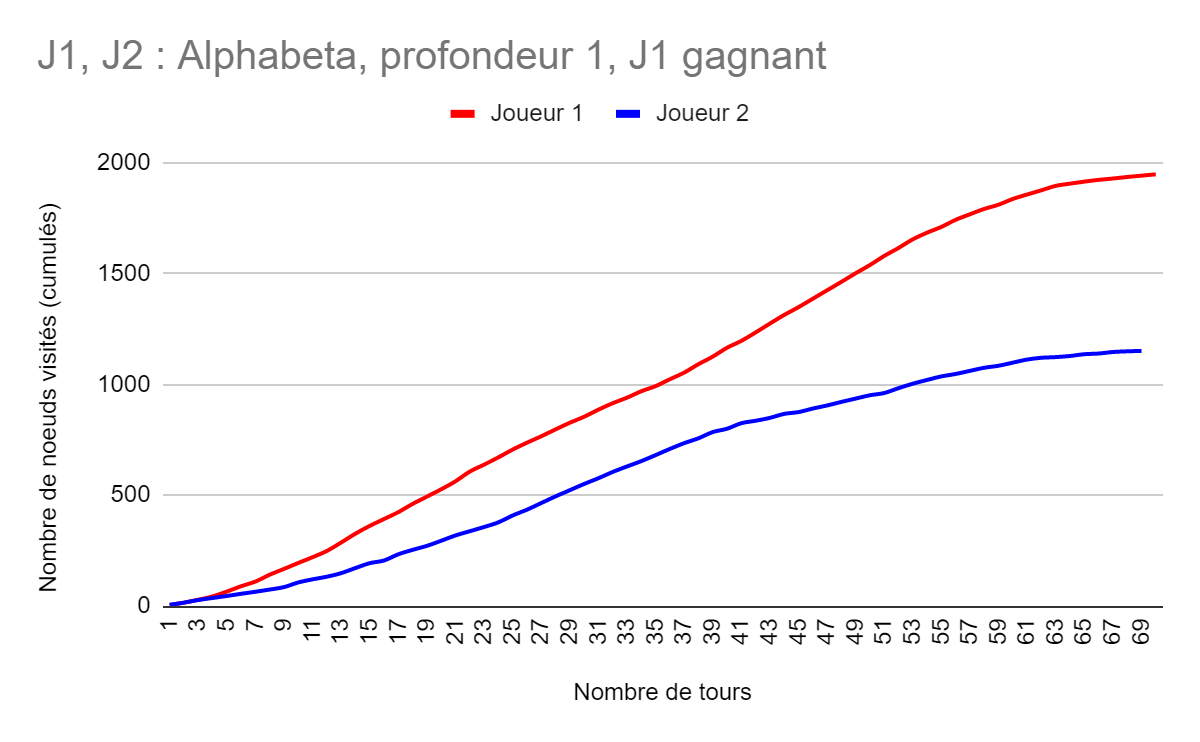
\includegraphics[width=\textwidth]{prof1alphabeta.png}
\end{figure}

Le joueur 1 obtient assez vite (tour 5) un avantage (il possède plus de possibilités) qui augmente au fur et à mesure des tours. A son maximum (tour 20) cet avantage est 47\% plus important par rapport au second joueur.\\
Cependant, c'est le second joueur qui gagne la partie.\\

L’augmentation de la complexité est plutôt linéaire.\\
Il semblerait que jouer en deuxième apporte un avantage.
\newpage
\subsubsection{Profondeur 2}

\begin{figure}[!h]
   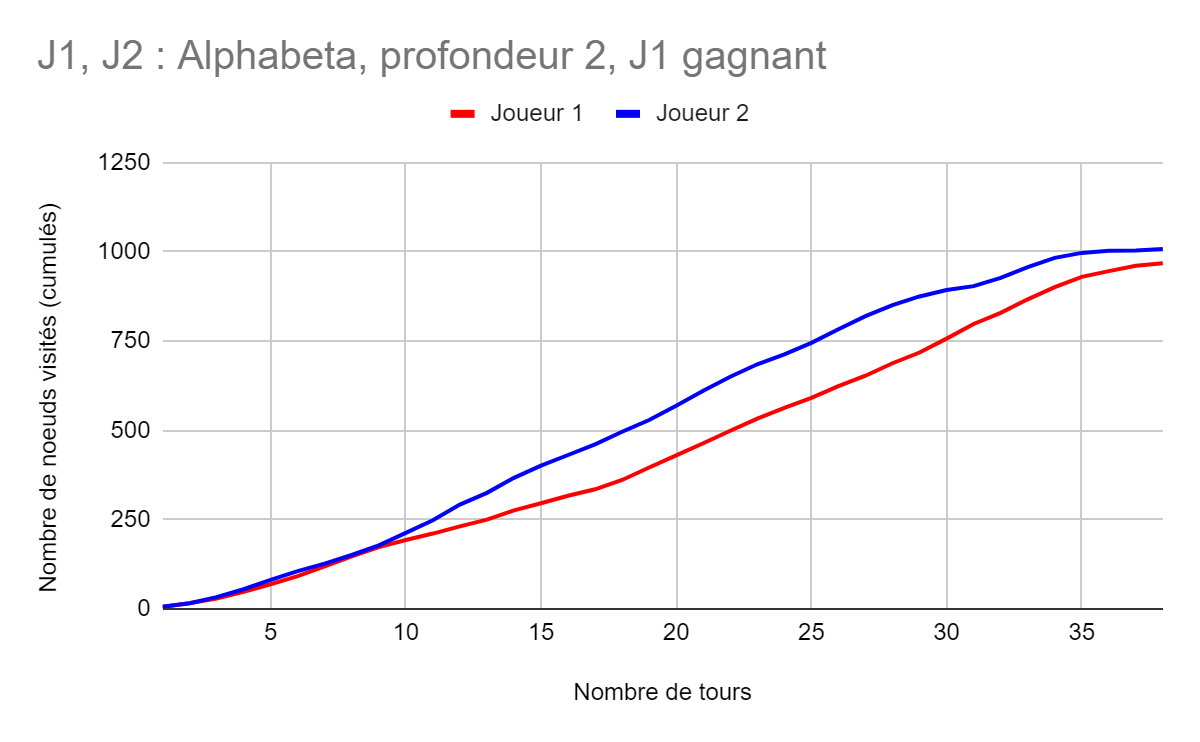
\includegraphics[width=\textwidth]{prof2alphabeta.png}
\end{figure}

Malgré qu’il soit second à jouer, le joueur 2 obtient un avantage au niveau du tour 5 environ. Cet avantage augmente jusqu’au tour 30, avec un pic à 79\% par rapport au joueur 1. Il se réduit ensuite jusqu’à la fin de la partie.\\
Le nombre de tours est largement inférieur par rapport au précédent graphique. La complexité du joueur 1 est deux fois moins importante que sur le graphique précédent, malgré la profondeur plus importante.\\
Mais malgré cet avantage, la victoire est pour le joueur 1.\\

La courbe est linéaire, comme sur le graphique précédent.\\
Être le premier à jouer semble donner un avantage, et le nombre de possibilités du joueur 2 plus important n’est pas suffisant pour le résorber. La profondeur ne semble pas forcément augmenter le nombre de possibilités.
\newpage
\subsubsection{Profondeur 3}

\begin{figure}[!h]
   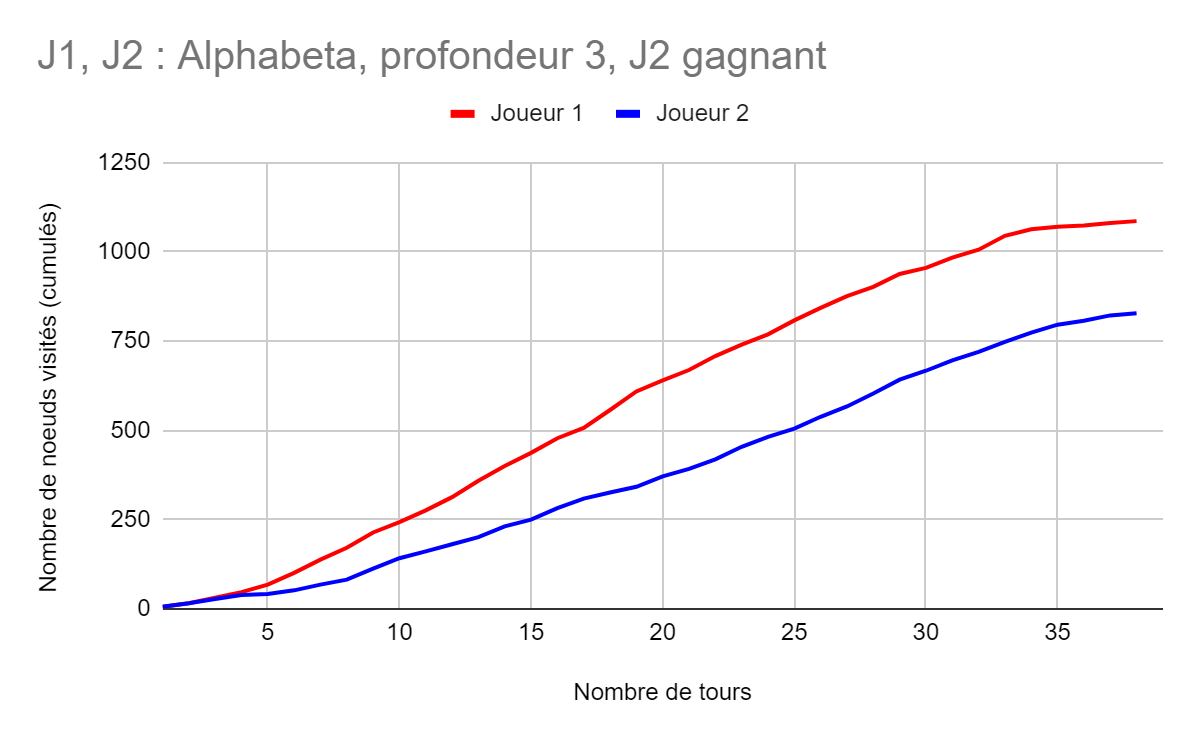
\includegraphics[width=\textwidth]{prof3alphabeta.png}
\end{figure}

Comme pour la profondeur 1, le joueur 1 a tôt, au tour 5 environ, un avantage qui augmente également au fur et à mesure de la partie. Cet avantage atteint un pic au tour 25 avec 60\% par rapport au second joueur.\\
Cependant, c'est le second joueur qui l'emporte, malgré son nombre de possibilités de jeu moins important.\\

Comme précédemment la courbe est plutôt linéaire.\\
La profondeur plus importante de l'algorithme n'augmente pas le nombre de tours de la partie.\\
Jouer en premier n'est pas obligatoirement avantageux.
\newpage
\subsubsection{Profondeur 4}

\begin{figure}[!h]
   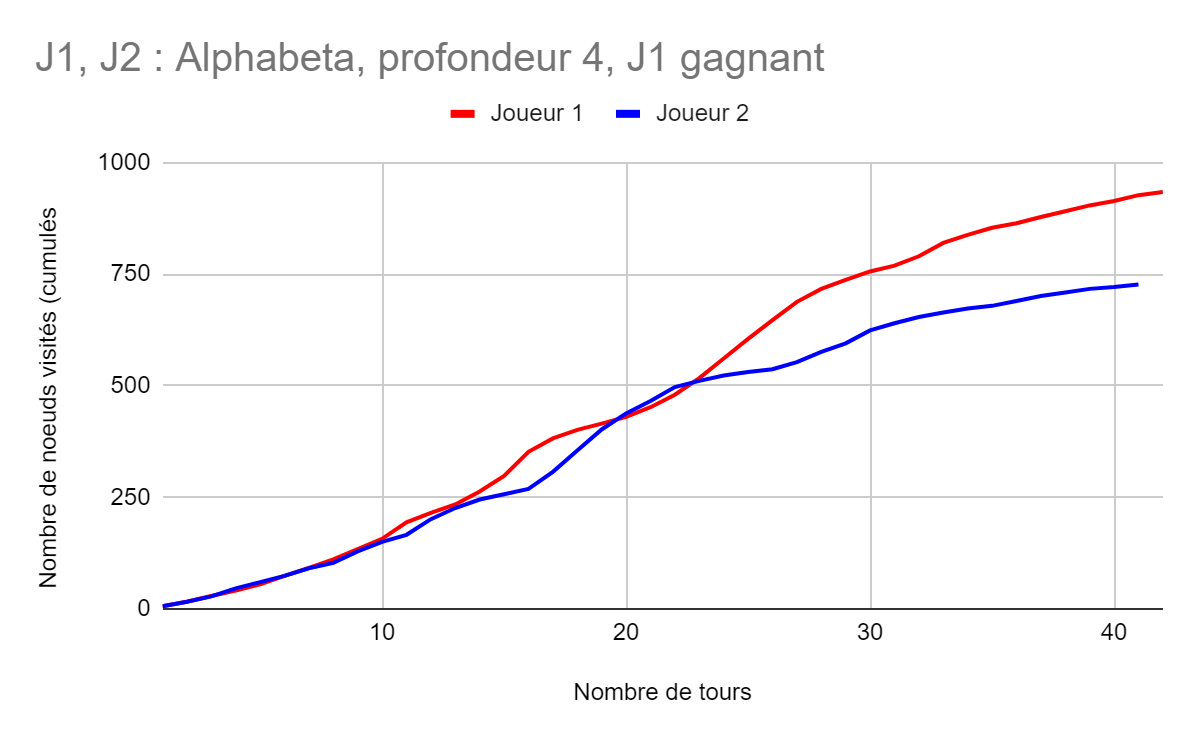
\includegraphics[width=\textwidth]{prof4alphabeta.png}
\end{figure}

Le premier joueur possède un petit avantage à partir du tour 10 environ. Mais au tour 18, cet avantage se réduit, pour réaugmenter au tour 23 jusqu'à la fin de partie. Il atteint au maximum 28\% par rapport au joueur 2.\\
C'est le premier joueur qui remporte la partie.\\

Comme précédemment, la courbe est plutôt linéaire. Le nombre de tours est similaire à l'algorithme de profondeur inférieur.\\
Sans avantage, le joueur 2 ne semble pas pouvoir renverser la tendance et doit s'incliner.
\newpage
\begin{figure}[!h]
   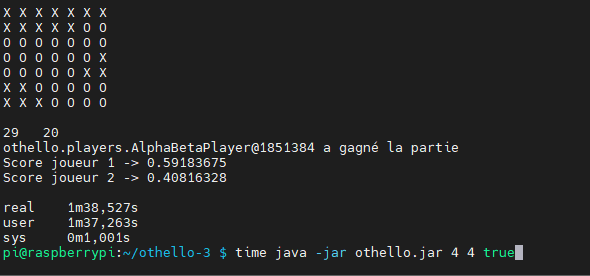
\includegraphics[width=\textwidth]{prof4alphabeta-console.png}
\end{figure}

Le temps de résolution de cet algorithme est de 1 minute et 38 secondes pour un total de 1 661 nœuds visités (pour les deux joueurs).

\newpage
\subsubsection{Profondeur 5}

\begin{figure}[!h]
   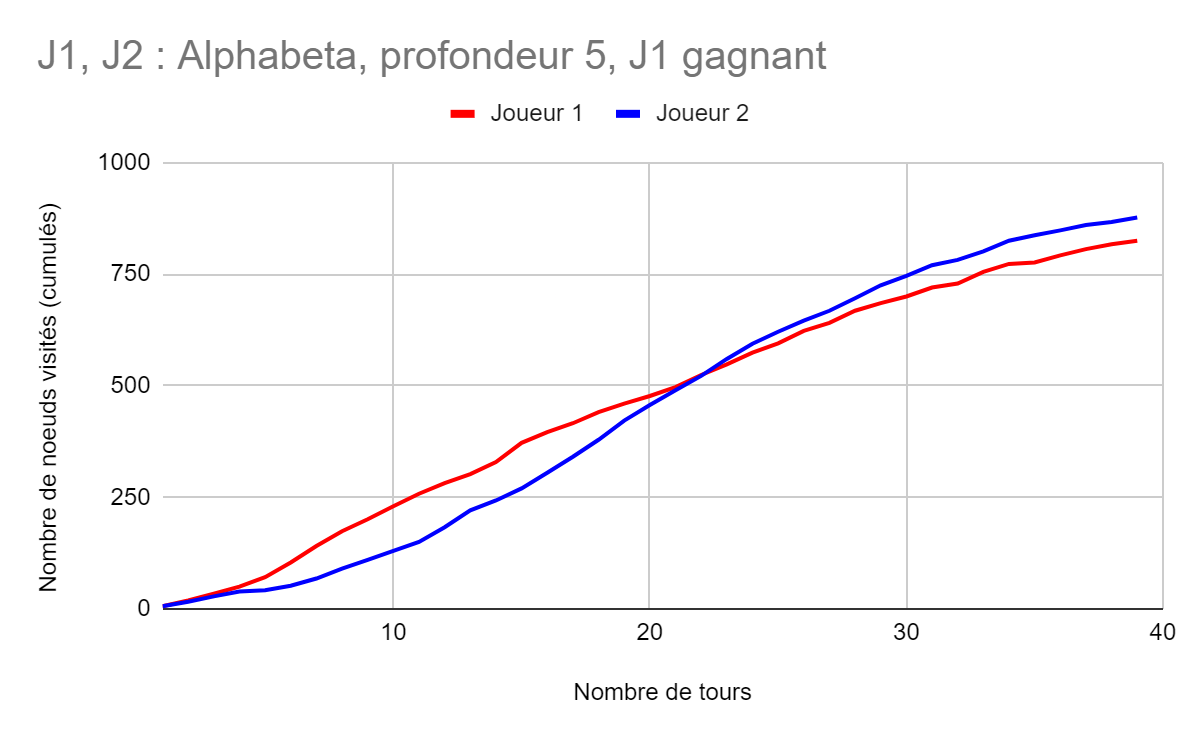
\includegraphics[width=\textwidth]{prof5alphabeta.png}
\end{figure}

Au tour 5 environ, le premier joueur obtient un léger avantage qui se résorbe au tour 22.\\
Ensuite, c'est le second joueur qui gagne un petit avantage qui se maintient jusqu'à la fin de la partie .\\
Malgré l'avantage du joueur 2 à la fin, c'est le joueur 1 qui l'emporte.\\

Identique au précédent graphique, la courbe est plutôt linéaire et le nombre de tours n'augmente pas.\\
L'avantage du second joueur sur la fin de la partie ne semble pas suffisant pour l'emporter.
\newpage
\begin{figure}[!h]
   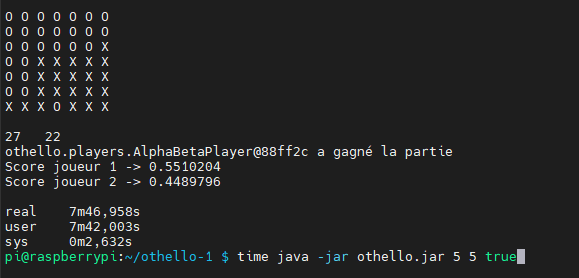
\includegraphics[width=\textwidth]{prof5alphabeta-console.png}
\end{figure}

Pour 1 702 nœuds visités, l’algorithme dure 7 minutes et 47 secondes. 

\subsubsection{Conclusion d’Alphabeta}

L'ordre n'est pas un avantage.
Le second joueur surpasse des fois le premier joueur, alors qu'il n'a pas de réel avantage. En effet, alors qu'il avait 60\% de possibilité en moins par rapport au premier joueur, le second l'a emporté avec l'algorithme Alphabeta de profondeur 3. Cas similaire avec Alphabeta de profondeur 1.
De plus, le second joueur possède un avantage de 79\% au maximum par rapport au premier joueur avec l'algorithme Alphabeta de profondeur 2. Et malgré cet avantage, c'est le joueur 1 qui remporte la partie.
Il semblerait que le nombre de possibilités n'influe pas sur la victoire avec cet algorithme, malgré ce qu'on pourrait logiquement penser.\\

L’augmentation de la profondeur de l’algorithme AlphaBeta n’augmente pas forcément la complexité de ce dernier. Cependant, l’augmentation de la complexité en fonction du nombre de tour est relativement linéaire.\\
Le temps de résolution des algorithmes pour des petites profondeurs (1, 2, 3) est de quelques secondes, mais augmente drastiquement avec la profondeur, AlphaBeta de profondeur 5 s’exécute durant plusieurs minutes. 

\newpage
\subsection{Negamax}

\subsubsection{Profondeur 1}

\begin{figure}[!h]
   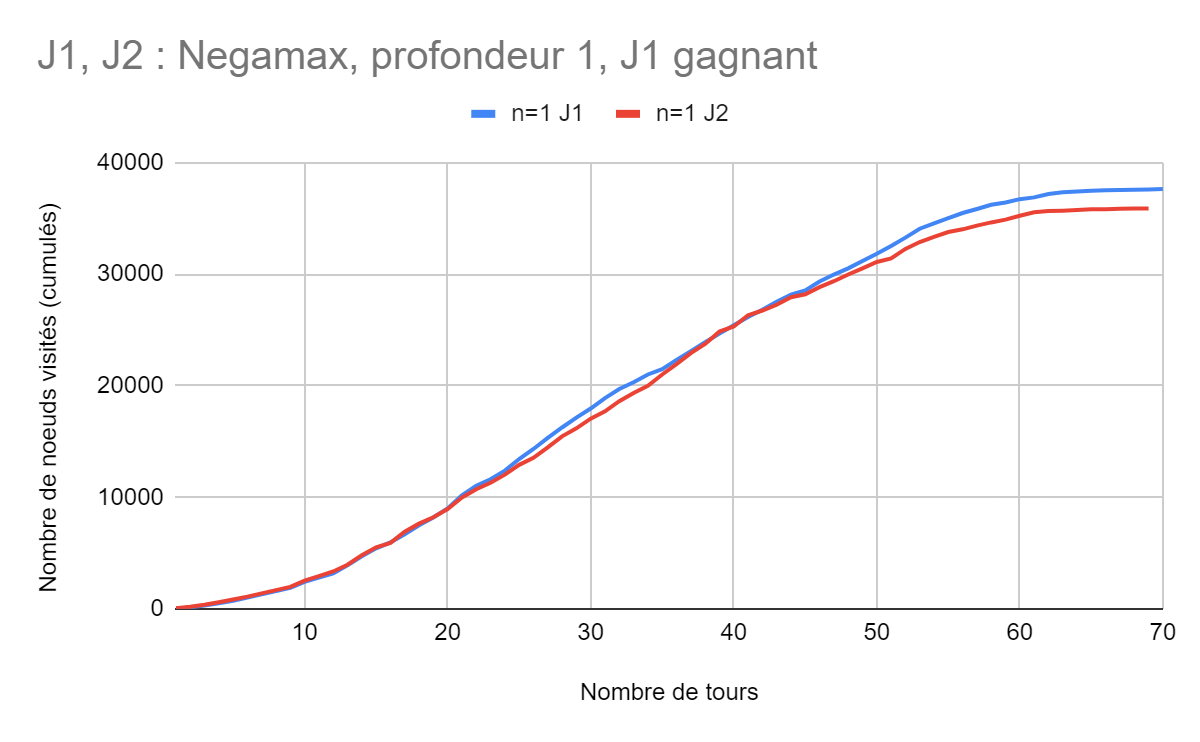
\includegraphics[width=\textwidth]{prof1negamax.png}
\end{figure}

Aucun des joueurs n’a d’avantage particulier.\\
La complexité est environ 30 fois plus importante qu’AlphaBeta.\\
Le joueur 2 est le gagnant. Avec cet algorithme, aussi, il semblerait que l'ordre ne soit pas un avantage.\\
L’augmentation de la complexité est moins importante au début et à la fin de partie, mais est assez linéaire.

\newpage
\subsubsection{Profondeur 2}

\begin{figure}[!h]
   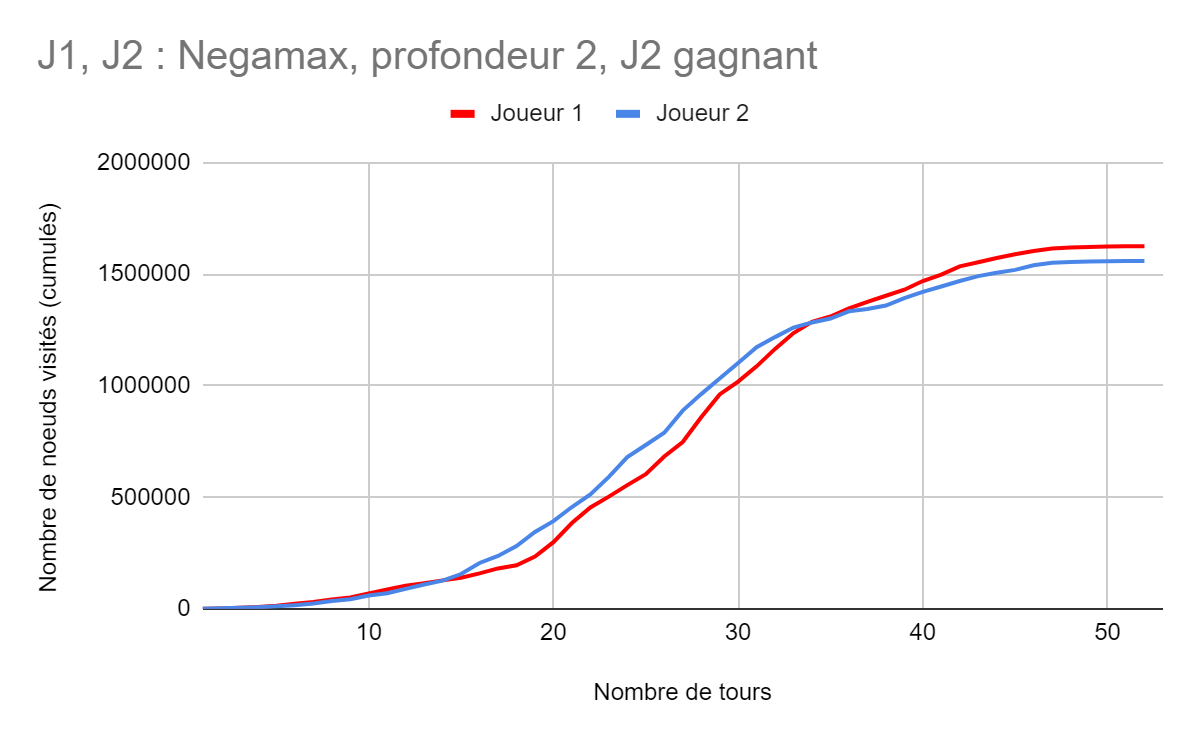
\includegraphics[width=\textwidth]{prof2negamax.png}
\end{figure}

La complexité est 20 fois plus importante qu’avec la profondeur précédente.\\
La forme de la courbe est similaire au graphique précédent.\\
Aucun joueur n’a d’avantage majeur au cours de la partie. Le second joueur a un avantage qui commence au tour 19 jusqu'à ka fin de la partie. Cet avantage atteint au maximum 37\% par rapport au joueur 1. \\
Cependant, c’est le premier joueur qui l’emporte, alors qu’il n’avait pas un grand avantage.

La complexité est bien plus importante qu'avec le précédent algorithme, mais le nombre de tours est plus petit.

\newpage
\subsubsection{Profondeur 3}

\begin{figure}[!h]
   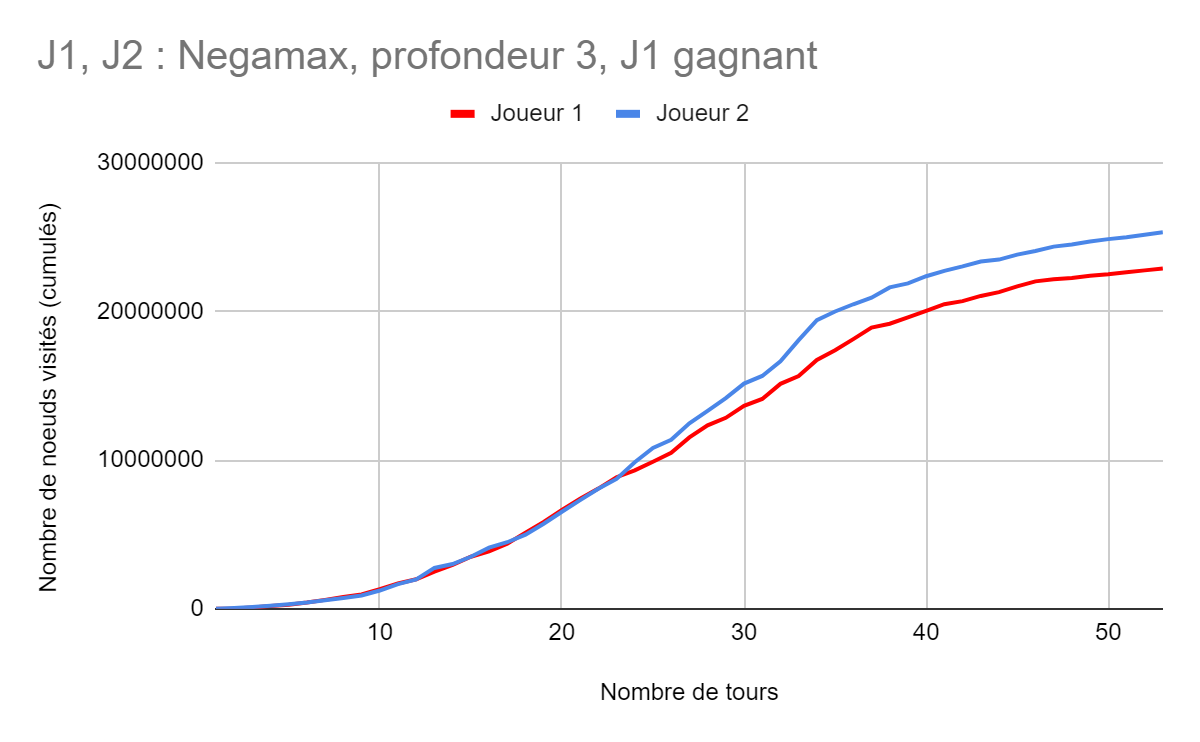
\includegraphics[width=\textwidth]{prof3negamax.png}
\end{figure}

La complexité de cet algorithme est 55 fois supérieure au précédent.\\
Le joueur 1 commence à avoir un avantage au tour 10, avantage qui augmente jusqu’à la fin de la partie. Cependant, cet avantage n’est pas suffisant et c’est le second joueur qui gagne.\\

Les courbes évoluent de façon similaire.
La complexité est bien plus grande qu'avec le précédent graphique, mais le nombre de tours est le même.

\newpage
\subsubsection{Profondeur 4}

\begin{figure}[!h]
   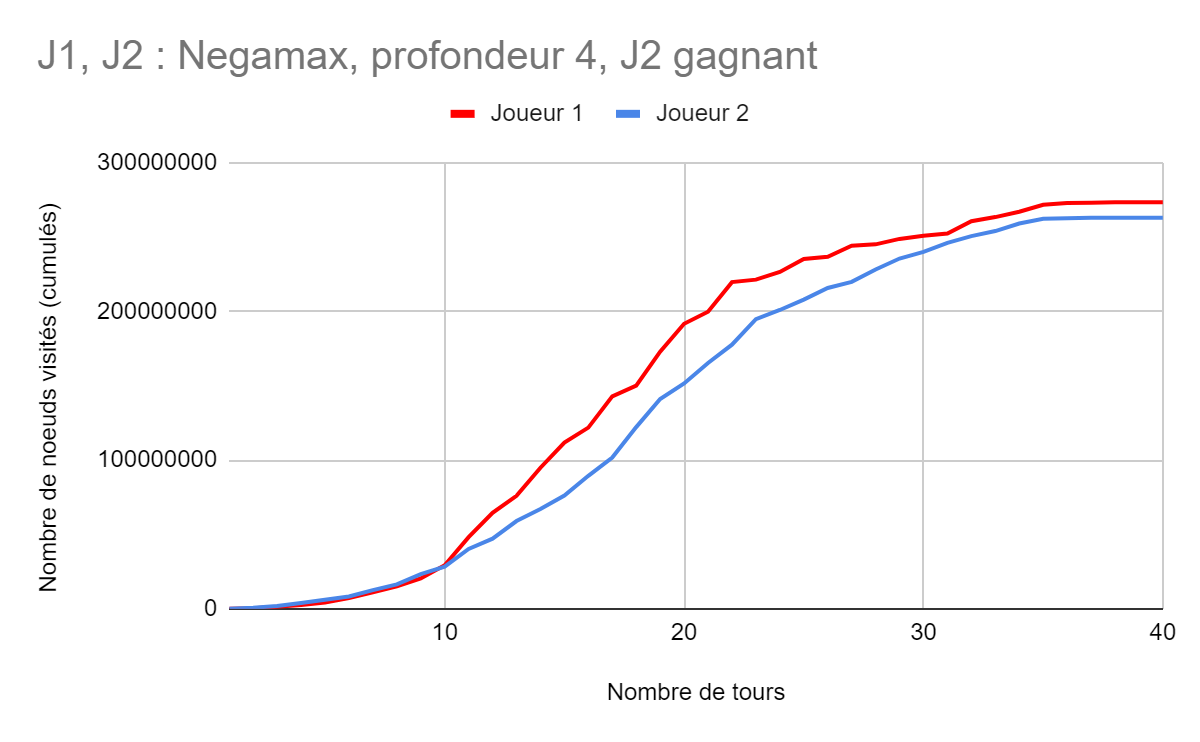
\includegraphics[width=\textwidth]{prof4negamax.png}
\end{figure}

La complexité est environ 10 fois supérieur à Negamax de profondeur 3. Le premier joueur possède un avantage au tour 10 qui augmente jusqu’au tour 22 et se réduit ensuite jusqu’à la fin de la partie.\\
Malgré cet avantage, c’est le second joueur qui remporte la partie.
\newpage
\begin{figure}[!h]
   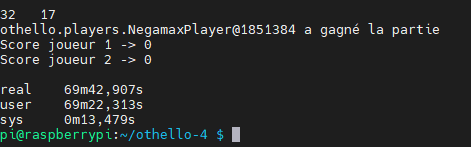
\includegraphics[width=\textwidth]{prof4negamax-console.png}
\end{figure}

Pour le parcours des 536 329 836 nœuds, l’algorithme met 70 minutes et 57 secondes. 

\subsubsection{Profondeur 5}

Nous avons estimé la complexité de Negamax de profondeur 5 à au moins 8.2 milliards de nœuds.\\
Nous avons é de le lancer, mais après 28 heures d’exécution sur le Raspberry Pi celui-ci n’étais pas terminé, de plus la complexité stockée comme attribut de la classe Player est stocké sur un entier signé 32 bits dont la limite positive est $2^{31} - 1$ soit inférieur à 8 milliards.
\newpage
\subsubsection{Conclusion de Negamax}

L’augmentation de la complexité en fonction de la profondeur de l’algorithme est exponentielle.\\
La victoire d’un joueur n’a pas l’air influé par son avantage ou par son ordre de jeu.\\
Dû à sa complexité exponentielle, le temps d’exécution de cet algorithme l’est également.
Cependant, le nombre de tours de jeu n'a pas l'air influé par la complexité de Negamax.

\newpage
\subsection{Negamax vs AlphaBeta}

\subsubsection{Profondeur 2, AlphaBeta premier joueur, Negamax second}

\begin{figure}[!h]
   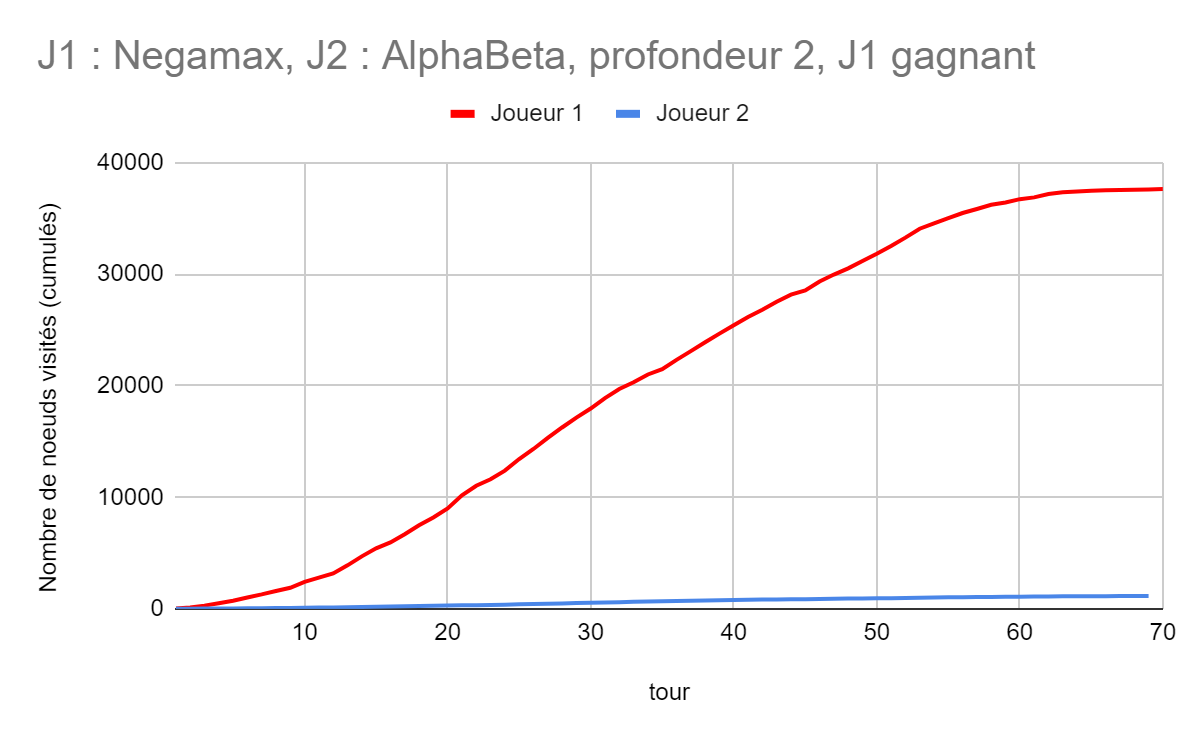
\includegraphics[width=\textwidth]{prof2alphaVSnegamax.png}
\end{figure}

Dès le premier tour, le joueur 2 avec l'algorithme Negamax, possède un très grand avantage qui augmente fortement par rapport au premier joueur.\\
Avec cet avantage, il gagne la partie, malgré qu'il soit second à jouer.

\newpage
\subsubsection{Profondeur 2, Negamax premier joueur, AlphaBeta second}

\begin{figure}[!h]
   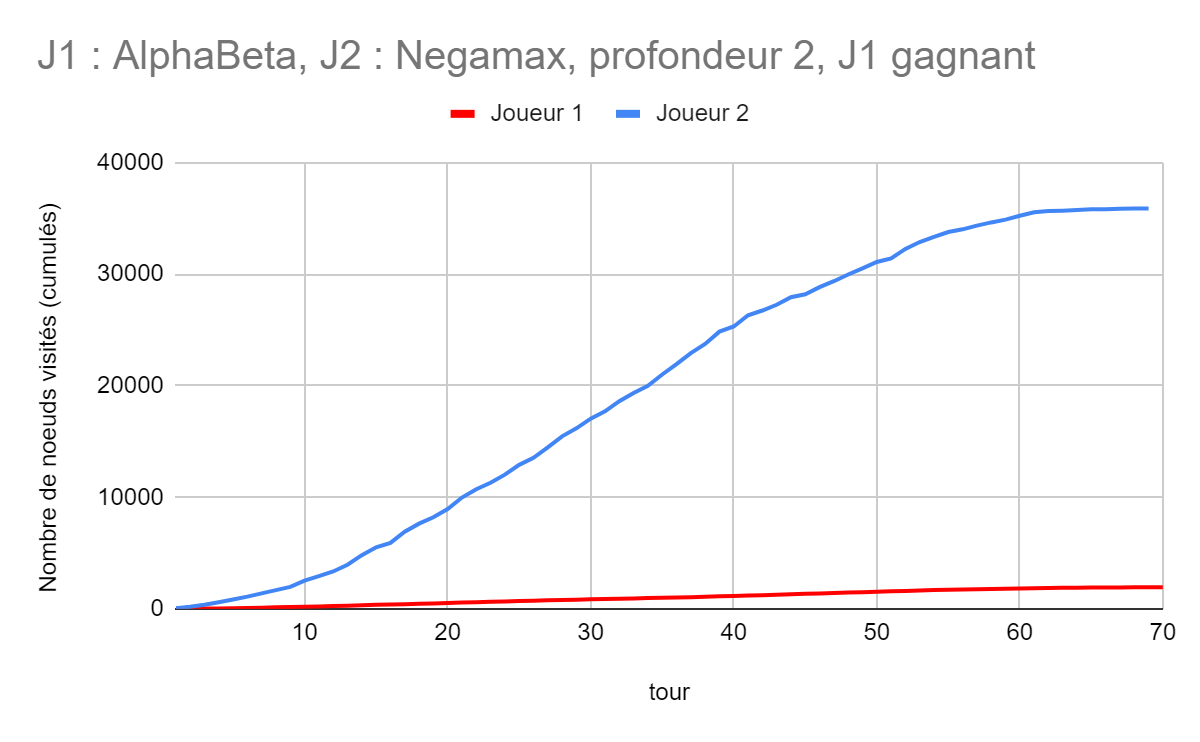
\includegraphics[width=\textwidth]{prof2negamaxVSalpha.png}
\end{figure}

Identiquement au graphique précédent, le premier joueur utilisant l'algorithme Negamax prend un avantage dès le premier tour. Son avantage augmente rapidement et se poursuit jusqu'à la fin de la partie pour enfin la remporter.

\subsubsection{Conclusion de AlphaBeta vs Negamax}

L'algorithme Negamax parcours beaucoup plus de noeud, il prend rapidement un très gros avantage.
Cet algorithme est plus efficace qu'AlphaBeta, mais il est plus long à exécuter.

\newpage
\section{Difficultés rencontrés}

Nous avons rencontré quelques difficultés durant la réalisation du jeu, notamment dû à des incompréhensions des règles du jeu:\\

\begin{itemize}
    \item Lors du clonage toutes les cases même inoccupées étaient modifiées.
    \item Le saut était possible même quand il n'y avait pas de pion en dessous et ne transformait pas les pions adverses.
\end{itemize}

\section{Expérimentations}

Nous avons mis en place un writer afin de pouvoir exporter plus facilement les données notamment pour faire les graphiques.\\

Le flux s'ouvre au lancement du programme et se ferme à sa fermeture ce qui fait que les fichiers de log resteront vides pendant le fonctionnement du programme, ce qui rend impossible la lecture de la complexité durant le fonctionnement du programme notamment pour le negamax de profondeur 5 ou plus qui demande beaucoup de performances et de temps de calcul.


\section{Conclusion}
\end{document}